\tableofcontents

%todo: thm = theorem
%todo: lm = lemma
%todo: def = definition
%todo: col = corollary

%================================
%::::::::::::::::::::::::::::::::
\chapter{Metric Spaces}
%::::::::::::::::::::::::::::::::
%================================


%================================
\section{Metric Spaces}
%================================



%--------------------------------
\begin{definition}
	\label{def: metric axioms}
	Let $X$ be any set.
	
	A function $d: X \times X \to \mathbb R_{\ge 0}$ is \textit{metric function}, or, simply, \textit{metric on $X$} iff it satisfies the \textit{metric axioms}. That is, for any $x, y, z \in X$:
	\begin{enumerate}[\bf M1. ]
		\item $d(x,y) = 0$ iff $x = y$;
		\item $d(x,y) = d(y,x)$;
		\item $d(x, z) \le d(x,y) + d(y,z)$.
	\end{enumerate}
\end{definition}
%--------------------------------


%--------------------------------
\begin{definition}
	\label{def: metric space}
	Let $X$ be any set and let $d$ be a structure on $X$.
	
	The pair $(X, d)$ is called a \textit{metric space} iff $d$ is a metric on $X$.
\end{definition}
%--------------------------------


%--------------------------------
\begin{definition}
	\label{def: ball}
	A $\mathbb X = (X, d)$ be a metric space, let $x \in X$ and let $\varepsilon \in \mathbb R_{> 0}$.
	
	An \textit{open $\varepsilon$-ball}, or just $\varepsilon$-ball, about $x$ is defined to be the set
	$$
	B_\varepsilon (x; d) := \{ y \in X : d(x,y) < \varepsilon \}.
	$$
	
	A \textit{closed ball} is defined to be the set
	$$
	\overline{B}_\varepsilon (x; d) := \{ y \in X : d(x,y) \le \varepsilon \}.
	$$
\end{definition}
%--------------------------------


%--------------------------------
\begin{note}
	As
	$$
	\mathbb X_0 = (X, d_0), \ \mathbb X_1 = (X, d_1), \ \mathbb X_2 = (X, d_2), \ \ldots
	$$
	are different although they share the same set $X$, for any $x \in X$ and any $\varepsilon \in \mathbb R_{> 0}$,
	$$
	B_\varepsilon(x; d_1),\ B_\varepsilon (x; d_2), \ B(x; d_3), \ \ldots
	$$
	are also different. However, if confusion is unlikely, we simply write ``$B_\varepsilon(x)$'' for ``$B_\varepsilon(x; d)$''.
\end{note}
%--------------------------------


%--------------------------------
\begin{example}
	The \textit{Euclidean metric space} $\mathbb X = (X, d)$ is an $n$-dimensional set $X$ equipped with the \textit{Euclidean metric} $d$ defined as
	$$
	d(x,y) := \left( \sum_{i = 1}^n |x_i - y_i|^2 \right)^\frac{1}{2}.
	$$
	
	This is also called \textit{standard Euclidean metric}, in contrast to the \textit{non-standard Euclidean metrics}
	$$
	d_p(x,y) := \left( \sum_{i = 1}^n |x_i - y_i|^p \right)^\frac{1}{p}, \quad p \ge 1.
	$$
	
	In particular,
	$$
	d_\infty (x,y) := \max_{1 \le i \le n} |x_i - y_i|.
	$$
\end{example}
%--------------------------------


%--------------------------------
\begin{example}
	A \textit{discrete metric space} $\mathbb X = (X, d)$ is a set $X$ equiped with the \textit{discrete metric} $d_\mathrm{dsic}$ defined as
	$$
	d_\mathrm{disc}(x,y) :=
	\begin{cases}
		0, & \text{if $x = y$}; \\
		1, & \text{else}.
	\end{cases}
	$$
	
	This is an equivalent definition of the discrete metric:
	$$
	d_\mathrm{disc}(x, y) := (\mathrm{sgn}(d(x,y)))^2,
	$$
	where $\mathrm{sgn}(\cdot)$ is a \href{https://en.wikipedia.org/wiki/Sign_function}{sign function}, and $d$ is any metric on $X$.
\end{example}
%--------------------------------


%--------------------------------
\begin{example}
	\footnote{
		See \href{https://en.wikipedia.org/wiki/Minkowski_inequality}{Minkowski inequality}.
	}
	Let $\mathbb I = (C{[a,b]}, d_p)$ be a metric space where $C{[a,b]}$ denotes the set of all continuous mapping $\mathbb R_{[a,b]} \to \mathbb R$, and $p > 0$, and the metric $d_p$ is defined as
	$$
	d_p(f, g) := \left( \int_{a}^{b} |f(t) - g(t)|^p \mathrm{d} t \right)^\frac{1}{p}.
	$$
	
	In particular,
	$$
	d_\infty (f,g) := \sup_{t \in \mathbb R_{[a,b]}} |f(t) - g(t)|.
	$$
\end{example}
%--------------------------------


%--------------------------------
\begin{example}
	\footnote{
		See \href{https://en.wikipedia.org/wiki/Hausdorff_distance}{Hausdorff distance}.
	}	
	Let $\mathbb X = (X, d)$ be a metric space. The \textit{Hausdorff metric} $d_H$ on $2^X \setminus \{\emptyset\}$ is defined as
	$$
	d_H := \max \left\{ \sup_{x \in X}d(x,Y), \sup_{y \in Y} d(y, X)\right\},
	$$
	where
	$$
	\begin{aligned}
		d(x,Y) := \inf_{y \in Y}(x,y), \text{ and } d(y, X) := \inf_{x \in X} (y, x).
	\end{aligned}
	$$
\end{example}
%--------------------------------


%================================
\section{Open Sets in Metric Spaces}
%================================


%--------------------------------
\begin{definition}
	\label{def: open set in metric space}
	Let $\mathbb X = (X, d)$ be a metric space, and let $U \subseteq X$.
	
	$U$ is said to be \textit{open in $\mathbb X$}, iff for any $y \in U$, there exists $\varepsilon \in \mathbb R_{> 0}$, such that $B_\varepsilon(y) \subseteq U$.
\end{definition}
%--------------------------------


%--------------------------------
\begin{proposition}
	\label{prop: open balls of point inside open ball}
	Let $\mathbb X = (X, d)$ be a metric space, let $x \in A$ and let $\varepsilon \in \mathbb R_{> 0}$.
	
	For any $y \in B_\varepsilon (x)$, there is a $\delta \in \mathbb R_{> 0}$ such that $B_\delta (y) \subseteq B_\varepsilon(x)$.
	
	\begin{proof}
		For any $y \in B_\varepsilon (x)$, by the definition of open balls (Definition \ref{def: ball}), we have $d(x,y) < \varepsilon$.
		
		Let $\delta \in \mathbb R_{> 0}$ such that $\delta + d(x,y) = \varepsilon$.
		
		By M3 in metric axioms (Definition \ref{def: metric axioms}), for any $z \in A$ with $d(y,z) < \delta$, we have
		$$
		d(x, z) \le d(y, z) + d(x, y) < \varepsilon.
		$$
		
		Thus, again, by the definition of open balls, we have $B_\delta(y) \subseteq B_\varepsilon(x)$.
		
		\qed
	\end{proof}
\end{proposition}
%--------------------------------


% Shared on Proof Wiki
% https://proofwiki.org/wiki/Set_is_Open_iff_Union_of_Open_Balls}{ProofWiki
%--------------------------------
\begin{proposition}
	\label{prop: set is open iff union of open balls}
	Let $\mathbb X = (X, d)$ be a metric space, and let $U \subseteq X$.
	
	$U$ is open in $\mathbb X$ iff it is a union of open balls.
	
	\begin{proof}
		First, prove $\Rightarrow$.
		
		As $U$ is open, for any $y \in U$, there exists $\varepsilon_y \in \mathbb R_{> 0}$ such that $B_{\varepsilon_y}(y) \subseteq U$.
		
		Therefore,
		$$
		U = \bigcup_{y \in U} B_{\varepsilon_y} (y).
		$$
		
		$\qedlm$
		
		Now, prove $\Leftarrow$.
		
		Aiming for a contradiction, suppose $U$ is a union of open balls but not open.
		
		As $U$ is not open, there is a $y \in U$ such that for any $\varepsilon \in \mathbb R_{> 0}$, $B_\varepsilon (y) \not \subseteq U$.
		
		As $U$ is a union of open balls, there is an $x \in U$ and $r \in \mathbb R_{> 0}$ such that $y \in B_r (x)$.
		
		By Proposition \ref{prop: open balls of point inside open ball}, there exists a $\delta \in \mathbb R_{> 0}$ such that $B_\delta (y) \subseteq B_r (x)$.
		
		This is a contradiction by the assumption.
		
		Thus, $U$ has to be open.
		
		\qed
	\end{proof}
\end{proposition}
%--------------------------------


% Shared on ProofWiki
% https://proofwiki.org/wiki/Metric_Space_is_Hausdorff
%--------------------------------
\begin{proposition}
	\label{prop: metric space is hausdorff}
	Let $\mathbb X = (X, d)$ be any metric space.
	
	$\mathbb X$ is \textit{Hausdorff}. That is, For any distinct points $x,y \in X$, we can always find an $\varepsilon \in \mathbb R_{> 0}$ such that
	$$
	B_\varepsilon(x) \cap B_\varepsilon(y) = \emptyset.
	$$
	
	\begin{proof}
		Aiming for a contradiction, suppose there are $x,y \in X$ with $x \ne y$, such that for any $\varepsilon \in \mathbb R_{> 0}$, we can always find a $z \in X$ such that
		$$
		z \in B_\varepsilon(x) \cap B_\varepsilon(y).
		$$
		
		Let $r = d(x,y)/2$, and let $z \in B_r(x) \cap B_r(y)$.
		
		As $z \in B_r(x)$, by the definition of open balls (Definition \ref{def: ball}), $d(x,z) < r$; as $z \in B_r(y)$, similarly, $d(y,z)< r$. Then we have
		$$
		d(x, z) + d(y, z) < 2r = d(x,y).
		$$
		
		This contradicts the metric axioms M3 (Definition \ref{def: metric axioms}).
		
		Thus $\mathbb X$ is Hausdorff.
		
		\qed
	\end{proof}
\end{proposition}
%--------------------------------


%--------------------------------
\begin{definition}
	\label{def: closed set in metric space}
	Let $\mathbb X = (X, d)$ be any metric space, and let $V \subseteq X$.
	
	$V$ is said to be \textit{closed} in $\mathbb X$, iff there is an open set $U$ satisfies $X \setminus U = V$.
\end{definition}
%--------------------------------


%--------------------------------
\begin{proposition}
	\label{prop: singleton in metric space is closed}
	In a metric space, any singleton is closed.
	
	\begin{proof}
		Let $\mathbb X =(X, d)$ be a metric space, let $x \in X$, and let $y \in X \setminus \{x\}$.
		
		As $M$ is Hausdorff (Proposition \ref{prop: metric space is hausdorff}), there is an $\varepsilon \in \mathbb R_{> 0}$ such that
		$$
		0 < \varepsilon < d(x,y),
		$$
		thus $X \setminus \{x\}$ is open, hence, by Definition \ref{def: metric axioms}, its complement $\{x\}$ is open.
		
		\qed
	\end{proof}
\end{proposition}
%--------------------------------


% Shared on ProofWiki
% https://proofwiki.org/wiki/Finite_Intersection_of_Open_Sets_of_Metric_Space_is_Open
%--------------------------------
\begin{proposition}
	Let $\mathbb X = (X, d)$ be a metric space, denote $\mathcal T$ for the family of open subsets of $X$.
	
	Then $\mathcal T$ satisfies the following conditions:
	
	\begin{enumerate}[\bf O1.]
		\item $X, \emptyset \in \mathcal T$;
		\item For any $\mathcal U \subseteq \mathcal T$, $\bigcup \mathcal U \in \mathcal T$; in words, $\mathcal T$ is closed under arbitrary union;
		\item For any finite $\mathcal V \subseteq \mathcal T$, $\bigcap \mathcal V \in \mathcal T$; in words, $\mathcal T$ is closed under finite intersection.
	\end{enumerate}
	
	\begin{proof} \
		\begin{enumerate}[\bf O1.]
			\item
				As $\emptyset$ is the subset of any set, $\emptyset \in \mathcal T$. $\bigcup \emptyset = \emptyset \in \mathcal T$.
			
				By Definition \ref{def: closed set in metric space}, $X = X \setminus \emptyset$.
				
				\qedlm
				
			\item 
				Let $\mathcal U \subseteq \mathcal T$, and denote $\mathcal O$ for the open balls in $M$.
			
				For any $U \in \mathcal U$, there is an $\mathcal O_U \subseteq \mathcal O$ such that $U = \bigcup \mathcal O_U$. 
				
				Then we have
				$$
				\bigcup \mathcal U = \bigcup_{U \in \mathcal U} \left( \bigcup \mathcal O_U \right) = \bigcup_{U \in \mathcal U} \mathcal O_U.
				$$
				
				By Proposition \ref{prop: set is open iff union of open balls}, $\bigcup \mathcal U$ is open.
				
				\qedlm
				
			\item
				Let $\mathcal V$ be a finite subset of $\mathcal T$.
				
				Aiming for a contradiction, suppose $\bigcap \mathcal V$ is not open.
				
				By Definition \ref{def: open set in metric space}, there exists a $y \in \bigcap \mathcal V$ such that for any $\varepsilon \in \mathbb R_{> 0}$, $B_\varepsilon(y) \setminus \bigcap \mathcal V \ne \emptyset$.
				
				By De Morgan's law, we have
				$$
				\bigcup_{V \in \mathcal V}(B_\varepsilon (y) \setminus V) \ne \emptyset.
				$$
				
				Thus, there exists $V \in \mathcal V$ such that $B_\varepsilon (y) \setminus V \ne \emptyset$.
				
				As $V \in \mathcal T$ and $\varepsilon$ is arbitrarily given, by Proposition \ref{prop: open balls of point inside open ball}, $y \notin V$. This is a contradiction.
				
				Thus, $\bigcap \mathcal V$ is open.
				
				\qedlm
		\end{enumerate}
		
		Thus, the theorem is proved.
		
		\qed
	\end{proof}
\end{proposition}
%--------------------------------


%--------------------------------
\begin{proposition}
	Infinite intersections of open sets in some metric spaces are not necessarily open.
	
	\begin{proof}
		Consider $\mathbb R$ is a Euclidean metric space, and denote $\mathcal T$.
		
		Clearly, for any $n \in \mathbb N_{> 0}$ and for any $x \in X$, the open interval $B_{\frac{1}{n}}(x)$ is open, but
		$$
		\bigcap\left\{ B_{\frac{1}{n}}\left( x \right) : n \in \mathbb N_{> 0} \right\} = \{ x \} .
		$$
		
		For any $\varepsilon \in \mathbb R_{> 0}$, $B_\varepsilon(x) \setminus \{x\}$ is not empty, thus $\{x\}$ is not open.
		
		\qed
	\end{proof}
\end{proposition}
%--------------------------------


%================================
\section{Restrictions and Metric Subspaces}
%================================


Restriction of metric function is a useful tool to describe the relation between metric spaces with different sets but ``same'' metric function on the sets.

As a restriction of a relation $R$ on $X \times Y$ to a subset $A \times B \subseteq X \times Y$ is defined to be
$$
R \restriction_{A \times B} := R \cap (X \times Y),
$$
a restriction of a metric $d$ on a set $S$ to a subset $U \subseteq S$ is defined to be
$$
d \restriction_{(U \times U) \times \mathbb R_{> 0}} := d \cap ((U \times U) \times \mathbb R_{> 0}).
$$

If $B = Y$, customarily, we simply write $R \restriction_{A}$ for $R \restriction_{A \times B}$. Similarly, as the codomain of a metric function is alway $\mathbb R_{> 0}$, so we simply write $d \restriction_{U \times U}$ instead of $d \restriction_{(U \times U) \times \mathbb R_{> 0}}$.


%--------------------------------
\begin{definition}
	\label{def: subspace metric}
	Let $\mathbb X = (X, d)$ be a metric space, and let $A \subseteq X$.
	
	The \textit{metric on $A$ induced by $d$}, or the \textit{subspace metric of $d$ with respect to $A$} is defined to be
	$$
	d_A := d\restriction_{A \times A}.
	$$
\end{definition}
%--------------------------------


%--------------------------------
\begin{proposition}
	Let $\mathbb X = (X, d)$ be a metric space, and let $A \subseteq X$ and let $d_A := d\restriction_{A \times A}$.
	
	Then $\mathbb A = (A, d_A)$ is a metric space.
	
	\begin{proof}		
		As metric axioms (Definition \ref{def: metric axioms}) holds for any $x,y \in X$, and $A \subseteq X$, they also holds for any $a, b \in A$. As $d_A$ is the subspace metric of $d$ with respect to $A$, $d_A$ is a metric on $A$.
		
		Thus, $\mathbb A$ is a metric space.
	\end{proof}
\end{proposition}
%--------------------------------


%--------------------------------
\begin{definition}
	\label{def: metric subspace}
	Let $\mathbb X = (X, d)$ be a metric space, and let $A \subseteq X$. 
	
	$\mathbb A = (A, d_A)$ is a \textit{metric subspace} of $\mathbb X$ iff $d_A$ is a subspace metric of $d$ with respect to $A$.
\end{definition}
%--------------------------------



%================================
%::::::::::::::::::::::::::::::::
\chapter{Topological Spaces}
%::::::::::::::::::::::::::::::::
%================================


%================================
\section{Basic Definitions}
%================================


%--------------------------------
\begin{definition}
	\label{def: open set axioms}
	Let $X$ be any set, and let $\mathcal T \subseteq 2^X$.
	
	$\mathcal T$ is a \textit{topology on $X$} iff it satisfies the \textit{open set axioms}. That is,
	\begin{enumerate}[\bfseries O1.]
		\item $X \in \mathcal T$;
		\item For any $\mathcal U \subseteq \mathcal T$, $\bigcup \mathcal U \in \mathcal T$; in words, $\mathcal T$ is closed under arbitrary union.
		\item For any finite $\mathcal V \subseteq \mathcal T$, $\bigcap \mathcal V \in \mathcal T$; in words, $\mathcal T$ is closed under finite intersection.
	\end{enumerate}
	
	A subset $U \subseteq X$ is said to be \textit{open in $M$} iff it is an element of $\mathcal T$.
\end{definition}
%--------------------------------


%--------------------------------
\begin{definition}
	\label{def: topological space}
	Let $X$ be any set, and let $\mathcal T$ be a structure on $X$.
	
	The pair $(X, \mathcal T)$ is called a \textit{topological space} iff $\mathcal T$ is a topology on $X$.
\end{definition}
%--------------------------------


%--------------------------------
\begin{proposition}
	\label{prop: empty set is an element of topology}
	Let $\mathbb X = (X, \mathcal T)$ be a topological space.
	
	Then $\emptyset \in \mathcal T$.
	
	\begin{proof}
		As empty set is an element of any set, it also an element of $\mathcal T$.
		
		Therefore, we have
		$$
		\emptyset = \bigcup \emptyset \in \mathcal T.
		$$
		
		\qed
	\end{proof}
\end{proposition}
%--------------------------------


%--------------------------------
\begin{definition}
	\label{def: closed set}
	Let $\mathbb X = (X, \mathcal T)$ be a topological space.
	
	A subset $A \subseteq X$ is said to be \textit{closed in $\mathbb X$} iff there exists a $U \in \mathcal T$ such that $A = X \setminus U$.
\end{definition}
%--------------------------------


%--------------------------------
\begin{proposition}
	\label{prop: closed set axioms}
	Let $\mathbb X = (X, \mathcal T)$ be a topological space, and denote $\mathcal C$ for the family of all closed sets in $M$.
	
	Then $\mathcal C$ satisfies the following conditions:
	\begin{enumerate}[\bf C1.]
		\item $X, \emptyset \in \mathcal C$;
		\item For any $\mathcal A \subseteq \mathcal C$, $\bigcap \mathcal A \in \mathcal C$;
		\item For any finite $\mathcal B \subseteq \mathcal C$, $\bigcup \mathcal B \in \mathcal C$.
	\end{enumerate}
	
	\begin{proof}
		\begin{enumerate}[\bf C1.]
			\item
			As $\emptyset \in \mathcal T$ and $X = X \setminus \emptyset$, by Definition \ref{def: closed set}, $X$ is closed.
			
			Similarly, as $X \in \mathcal T$ and $\emptyset = X \setminus X$, $\emptyset$ is closed.
			
			\qedlm
			
			\item
			For any $\mathcal A \subseteq \mathcal C$, there exists a $\mathcal U \subseteq \mathcal T$ such that 
			$$
			\forall A \in \mathcal A: \exists U \in \mathcal U : A = X \setminus U. \quad
			\text{(Definition \ref{def: closed set}.)}
			$$
			Then we have
			$$
			\begin{aligned}
				\mathcal A = \left\{ X \setminus U : U \in \mathcal U \right\} &\iff \bigcap \mathcal A = \bigcap_{U \in \mathcal U} X \setminus U \\
				&\iff \bigcap \mathcal A = X \setminus \bigcup \mathcal U.
			\end{aligned}
			$$
			
			As $\bigcup \mathcal U \in \mathcal T$ by Definition \ref{def: open set axioms} O2, its complement $\bigcap \mathcal A \in \mathcal C$ by Definition \ref{def: closed set}.
				
				\qedlm
				
			\item
			For any finite $\mathcal B \subseteq \mathcal C$, there exists a finite $\mathcal U \subseteq \mathcal T$ such that
			$$
			\forall B \in \mathcal B: \exists U \in \mathcal U: A = X \setminus U. \quad
			(\text{Definition \ref{def: closed set}}.)
			$$
			Then we have
			$$
			\begin{aligned}
				\mathcal B = \{X \setminus U : U \in \mathcal U \} &\iff \bigcup \mathcal B =  \bigcup_{U \in \mathcal U} X \setminus U \\
				&\iff \bigcup \mathcal B = X \setminus \bigcap \mathcal U.
			\end{aligned}
			$$
			
			As $\bigcap \mathcal U \in \mathcal T$ by Definition \ref{def: open set axioms} O3, its complement $\bigcup \mathcal A \in \mathcal C$ by Definition \ref{def: closed set}.
			
			\qedlm
		\end{enumerate}
		
		Thus, the proof is done.
		
		\qed
	\end{proof}
\end{proposition}
%--------------------------------


%================================
\section{Some Important Topologies}
%================================


%--------------------------------
\begin{definition}
	\label{def: discrete topology}
	Let $X$ be any set.
	
	A family $\mathcal T \subseteq 2^X$ is a \textit{discrete topology on $X$} iff $\mathcal T = 2^X$.
\end{definition}
%--------------------------------


%--------------------------------
\begin{definition}
	\label{def: indiscrete topology}
	Let $X$ be any set.
	
	A family $\mathcal T \subseteq 2^X$ is an \textit{indiscrete topology on $X$} iff $\mathcal T = \{X, \emptyset\}$.
\end{definition}
%--------------------------------


%--------------------------------
\begin{definition}
	\label{def: induced topology}
	Let $\mathbb X = (X, d)$ be a metric space.
	
	A family $\mathcal T \subseteq 2^X$ is a \textit{topology induced by $d$} iff $\mathcal T$ is the set of all open sets in $\mathbb X$.
\end{definition}
%--------------------------------


%================================
\section{Comparison of Topologies}
%================================


%--------------------------------
\begin{definition}
	\label{def: comparison of topologies}
	Let $X$ be any set and let $\mathcal T_1$ and $\mathcal T_2$ be topologies on $X$.
	
	We say that $\mathcal T$ is \textit{coarser} than $\mathcal T_1$, or $\mathcal T_2$ is \textit{finer} than $\mathcal T_1$, iff $\mathcal T_1 \subseteq \mathcal T_2$.
\end{definition}
%--------------------------------


%--------------------------------
\begin{note}
	By the definition of cardinality and inclusion mapping, if $\mathcal T_1 \subseteq \mathcal T_2$, it is certainly true that $| \mathcal T_1 | \le | \mathcal T_2 |$. But, on the contrary, $| \mathcal T_1 | \le |\mathcal T_2|$ does not implies $\mathcal T_1 \subseteq \mathcal T_2$. It is easy to find counter-example about this.
\end{note}
%--------------------------------


%--------------------------------
\begin{example}
	By Definition \ref{def: comparison of topologies}, for any set $X$, if a family $\mathcal U$ of open sets is given, then we can find the coarsest topology on $X$ containing $\mathcal U$ by
	$$
	\mathcal T = \left\{ \bigcup \mathcal I, \bigcap \mathcal I, X : \mathcal I \subseteq \mathcal U \right\}.
	$$
	
	For example, let $X = \{1,2,3,4,5\}$, and let
	$$
	\mathcal U = \{\{1,2\}, \{2,3\}, \{4\}\}.
	$$
	Then a topology on $X$ contains at least these sets:
	$$
	\begin{matrix}
		\{1,2,3, 4\}, \{\}, \\
		\{1,2\}, \{2,3\}, \{4\}, \\
		\{1,2,3\}, \{1,2,4\}, \{2,3,4\}, \\
		\{2\}.
	\end{matrix}
	$$
\end{example}
%--------------------------------


%--------------------------------
\begin{example}
	The discrete topology is the finest topology on any $X$, while the indiscrete topology is the coarsest.
\end{example}
%--------------------------------


%================================
\section{Interiors}
%================================


%--------------------------------
\begin{definition}
	\label{def: interior}
	Let $\mathbb X = (X, \mathcal T)$ be a topological space, and let $A \subseteq X$.
	
	The \textit{interior} of $A$ is defined as
	$$
	\Int_{\mathcal T}(A) := \bigcup \left(\mathcal T \cap 2^A \right).
	$$
\end{definition}
%--------------------------------


%--------------------------------
\begin{note}
	Let $\mathbb X_1 = (X, \mathcal T_1)$, $\mathbb X_2 = (X, \mathcal T_2)$, and $A \subseteq X$. Then $\mathcal T_1 \ne \mathcal T_2$ iff $\Int_{\mathcal T_1}(A) \ne \Int_{\mathcal T_2}(A)$. In this case, the subscript for ``$\Int$'' is necessary.
	
	But, if the confusion is unlikely, we can also simply write $\Int (A)$ for $\Int_\mathcal T A$. In this case, it is also common to write $A^\circ$ for $\Int(A)$.
\end{note}
%--------------------------------


%--------------------------------
\begin{proposition}
	\label{prop: open iff interior}
	Let $\mathbb X = (X, \mathcal T)$ be a topological space, and let $A \subseteq X$.
	
	$A \in \mathcal T$ iff $A = A^\circ$.
	
	\begin{proof}
		First, prove $\Rightarrow$.
		
		If $A \in \mathcal T$, then we have
		$$
		\mathcal T \cap 2^A = \mathcal T \cap \{A\} \cap 2^A = \{A\} \cap 2^A = \{A\}.
		$$
		
		By Definition \ref{def: interior},
		$$
		A^\circ = \bigcup(\mathcal T \cap 2^A) = \bigcup\{A\} = A.
		$$
		
		\qedlm
		
		Now, prove $\Leftarrow$.
		
		By Definition \ref{def: interior}, we have
		$$
		A = \bigcup(\mathcal T \cap 2^A).
		$$
		
		As $\mathcal T \cap 2^A \subseteq \mathcal T$, thus, by open set axioms O2 (Definition \ref{def: open set axioms} O2), $A \in \mathcal T$.
		
		\qedlm
		
		Thus, the proof is done.
		
		\qed
	\end{proof}
\end{proposition}
%--------------------------------


%--------------------------------
\begin{proposition}
	\label{prop: point in open set}
	Let $\mathbb X = (X, \mathcal T)$ be a topological space, and let $A \in \mathcal T$. For any $x \in A$, there is a $U \in \mathcal T \cap 2^A$ such that $x \in U$.
	
	\begin{proof}
		$$
		\begin{aligned}
			% line 1
			x \in A &\iff x \in A^\circ
				% by
				&\text{(Proposition \ref{prop: open iff interior})} \\
			% line 2
			&\iff x \in \bigcup\left( \mathcal T \cap 2^A \right)
				% by
				&\text{(Definition \ref{def: interior})} \\
			% line 3
			&\iff \exists U \in \mathcal T \cap 2^A: x \in U.
		\end{aligned}
		$$
		
		\qed
	\end{proof}
\end{proposition}
%--------------------------------


%todo: >>>prove this<<<
%--------------------------------
\begin{proposition}
	\label{prop: union of intersection of family of families}
	Let $X$ be any set, let $I$ be an index set, and let $\mathcal A_i \subseteq 2^X$ for any $i \in I$.
	
	Then we have
	$$
	\bigcup \left( \bigcap_{i \in I} \mathcal A_i \right) \subseteq \bigcap_{i \in I} \left( \bigcup \mathcal A_i \right).
	$$
\end{proposition}
%%--------------------------------


\begin{figure}[h]
	\centering
    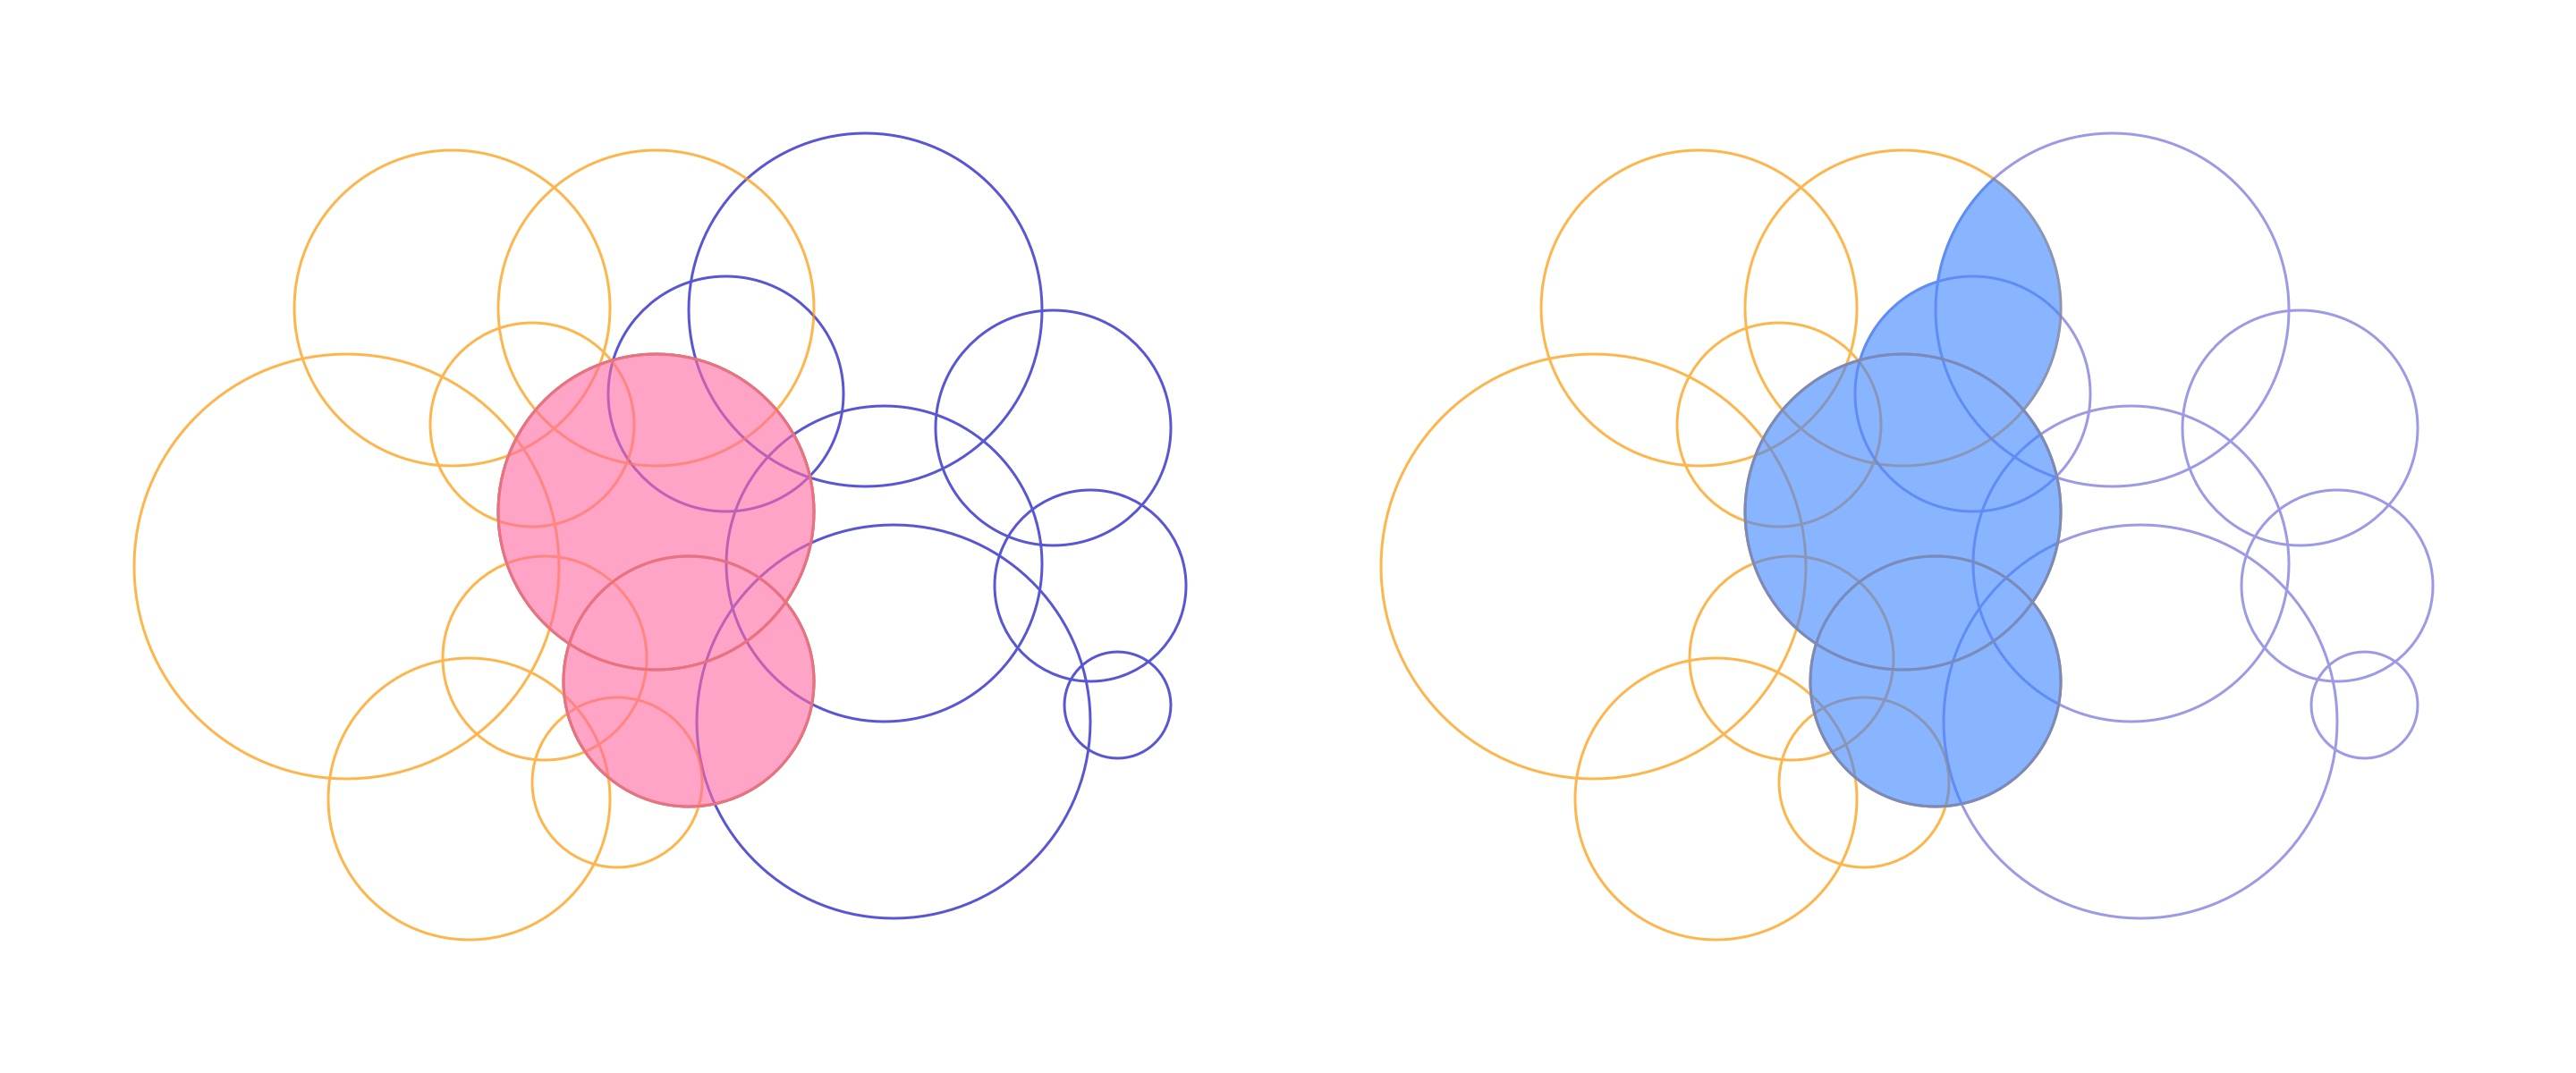
\includegraphics[width=345pt]{notes-for-general-topology/media/intersection-of-family-of-families}
    \caption{Diagram of the relation in Proposition \ref{prop: union of intersection of family of families}.}
\end{figure}




% Todo: Share on ProofWiki
% https://proofwiki.org/wiki/Intersection_of_Interiors_contains_Interior_of_Intersection
%--------------------------------
\begin{proposition}
	\label{prop: interior of intersection is a subset of intersection of interior}
	Let $\mathbb X = (X, \mathcal T)$ be a topological space, and let $\mathcal A \subseteq 2^X$.
	
	Then we have
	$$
	\left( \bigcap \mathcal A \right)^\circ \subseteq \bigcap_{A \in \mathcal A} A^\circ.
	$$
	
	\begin{proof}
		$$
		\begin{aligned}
			% line 1
			\left(\bigcap \mathcal A \right)^\circ &= \bigcup \left( \mathcal T \cap 2^{\bigcap \mathcal A} \right)
				% by
				&\text{(Definition \ref{def: interior})}
			\\
			% line 2
			&= \bigcup \left( \mathcal T \cap \bigcap_{A \in \mathcal A} 2^A \right)
				% by
				&\text{(\href{https://proofwiki.org/wiki/Intersection_of_Power_Sets}{intersection of power sets})}
			\\
			% line 3
			&= \bigcup \left( \bigcap_{A \in \mathcal A} \left(\mathcal T \cap 2^A \right) \right)
				% by
				&\text{(intersection is \href{https://proofwiki.org/wiki/Intersection_is_Idempotent}{idempotent}} \\
				&&\text{and \href{https://proofwiki.org/wiki/Intersection_is_Associative}{associative})}
			\\
			% line 4
			&\subseteq \bigcap_{A \in \mathcal A} \left( \bigcup \left( \mathcal T \cap 2^A \right) \right)
				% by
				&\text{(Proposition \ref{prop: union of intersection of family of families})}
			\\
			% line 5
			&= \bigcap_{A \in \mathcal A} A^\circ.
				% by
				&\text{(Definition \ref{def: interior})}
		\end{aligned}
		$$
		
		\qed
	\end{proof}
\end{proposition}
%--------------------------------


%--------------------------------
\begin{example}
	The equality in Proposition \ref{prop: interior of intersection is a subset of intersection of interior} may not hold.

	Let $\mathbb T = (\mathbb R, \mathcal T)$ be a topological space with
	$$
	\mathcal T = \{ X, (0,2), (1, 3), \emptyset \}.
	$$
	
	Then we have
	$$
	((0,2) \cap (1,3))^\circ = \emptyset \quad \subsetneq \quad (0,2)^\circ \cap (1,3) = (1,2).
	$$
\end{example}
%--------------------------------


%--------------------------------
\begin{proposition}
	\label{prop: inclusion implies interior inclusion}
	Let $\mathbb X = (X, \mathcal T)$ be a topological space, and let $A, B \subseteq X$.
	
	If $A \subseteq B$, then $A^\circ \subseteq B^\circ$.
	
	\begin{proof}
		$$
		\begin{aligned}
			% line 1
			A \subseteq B &\implies 2^A \subseteq 2^B
				% by
				&\text{(\href{https://proofwiki.org/wiki/Power_Set_of_Subset}{power set of subset})}\\
			% line 2
			& \implies \mathcal T \cap 2^A \subseteq \mathcal T \cap 2^B
				% todo: by what?
				& \\
			% line 3
			&\implies \bigcup(\mathcal T \cap 2^A) \subseteq \bigcup (\mathcal T \cap 2^B)
				% todo: by what?
				& \\
			% line 4
			&\implies A^\circ \subseteq B^\circ
				% by
				&\text{(Definition \ref{def: interior})}
		\end{aligned}
		$$
		
		\qed
	\end{proof}
\end{proposition}
%--------------------------------


%--------------------------------
\begin{note}
	Note that, $A^\circ \subseteq B^\circ$ does not implies $A \subseteq B$. Consider $\mathbb R$ as a Euclidean metric space, and let
	$$
	\begin{aligned}
		A = \{0\}, \quad B \subseteq \mathbb R \setminus \{0\}.
	\end{aligned}
	$$
	As $A^\circ = \emptyset$, $A^\circ \subseteq B^\circ$, but $A \setminus B = \{0\}$, so $A \not \subseteq B$.
\end{note}
%--------------------------------


%================================
\section{Limit Points and Isolated Points}
%================================


%--------------------------------
\begin{definition}
	\label{def: limit point}
	Let $\mathbb X = (X, \mathcal T)$ be a topological space, and let $A \subseteq X$.
	
	A point $x \in X$ is a \textit{limit point of $A$} iff for any $U \in \mathcal T$ with $x \in U$
	$$
	A \cap U \setminus \{x\} \ne \emptyset.
	$$
	
	The \textit{derived set of $A$} is the set of all limit points of $X$.
\end{definition}
%--------------------------------


%--------------------------------
\begin{definition}
	\label{def: isolated point}
	Let $\mathbb X = (X, \mathcal T)$ be a topological space, and let $A \subseteq X$.
	
	A point $x \in A$ is said to be \textit{isolated} iff there is $U \in \mathcal T$ with $x \in U$, such that
	$$
	A \cap U \setminus \{x\} = \emptyset.
	$$
\end{definition}
%--------------------------------


%--------------------------------
\paragraph{Notations.}
The Derived set of $A$ is usually denoted $A'$.\footnote{See \href{https://proofwiki.org/wiki/Definition:Derived_Set}{ProofWiki} and \href{https://en.wikipedia.org/wiki/Derived_set_(mathematics)}{Wikipedia}.}
But sometime it is also necessary to know in which space (with its topology) the derived set of $A$ is. For example, for topological spaces $\mathbb X_1 = (X, \mathcal T_1)$ and $\mathbb X_2 = (X, \mathcal T_2)$, if $\mathcal T_1 \ne \mathcal T_2$, the derived sets of a set $A$ in $\mathbb X_1$ and $\mathbb X_2$ may be different. So, below, the notation $A'$ is used only if the confusions are unlikely; else, we denote $\Li_\mathcal T A$ for $A'$ with respect to the topology $\mathcal T$.

Sometime, the set of isolated points of $A$ is denoted by $A^i$. For avoiding confusions, we denote $\I_\mathcal T(A)$ for $A^i$ with respect to the topology $\mathcal T$.
%--------------------------------


%--------------------------------
\begin{proposition}
	\label{prop: disjoint union of isolated set and derived set}
	Let $\mathbb X = (X, \mathcal T)$ be a topological space, and let $A \subseteq X$. 
	
	Then,
	$$
	A \subseteq \Li (A) \sqcup \I (A).
	$$
	
	\begin{proof}
		By Definition \ref{def: limit point}, $x \notin \Li(A)$ iff there exists a $U \in \mathcal T$ of $x \in U$ such that $A \cap N \setminus \{x\} = \emptyset$. This precisely satisfies Definition \ref{def: isolated point}. Thus
		$$
		A \subseteq \Li(A) \cup \I(A).
		$$
		
		As Definition \ref{def: limit point} and \ref{def: isolated point} are precisely logical complement for each other, $x \in \I (A) \cap \Li(A)$ always fails, i.e., $\I(A) \cap \Li(A) = \emptyset$. Thus
		$$
		A \subseteq \Li (A) \sqcup \I (A).
		$$
		
		\qed
	\end{proof}
\end{proposition}
%--------------------------------


%--------------------------------
\begin{proposition}
	\label{prop: closed iff contain all limit point}
	Let $\mathbb X = (X, \mathcal T)$ be a topological space, and let $A \subseteq X$.
	
	$A$ is closed iff $\Li(A) \subseteq A$.
	
	\begin{proof}
		First, prove $\Rightarrow$.
		
		Aiming for a contradiction, suppose $A$ is closed but there exists a $y \in \Li(A) \setminus A$.
		
		By Definition \ref{def: closed set}, as $A$ is closed, then $A^\complement$ is open.
		
		As $y \in A^\complement$ and $A^\complement$ is open, then, by Proposition \ref{prop: point in open set}, there exists a $U \in \mathcal T$ with $y \in U$, such that $U \subseteq A^\complement$.
		
		As $U$ is an open set containing $y$ and $A \cap U \setminus \{y\} = \emptyset$, then $y \notin \Li(A)$. This contradicts the assumption.
		
		Thus $\Li(A) \subseteq A$.
		
		\qed
	\end{proof}
\end{proposition}
%--------------------------------


%================================
\section{Closures}
%================================


%--------------------------------
\begin{definition}
	\label{def: closure}
	Let $\mathbb X = (X, \mathcal T)$ be a topological space, and let $A \subseteq X$.
	
	The \textit{closure of $A$} is defined as
	$$
	\Cl_\mathcal T(A) := A \cup \Li(A).
	$$
	
	When the confusions are unlikely, we simply write $\Cl(A)$, $\overline A$ or $A^-$ for $\Cl_\mathcal T(A)$.
\end{definition}
%--------------------------------


%--------------------------------
\begin{proposition}
	\label{prop: closed iff closure}
	Let $\mathbb X = (X, \mathcal T)$ be a topological space, and let $A \subseteq X$.
	
	$A$ is closed iff $A = A^-$
	
	\begin{proof}
		$$
		\begin{aligned}
			% \line 1
			A \text{ is closed} &\iff A \supseteq \Li(A)
				% by
				&\text{(Proposition \ref{prop: closed iff contain all limit point})}\\
			% \line 2
			&\iff A = A \cup \Li(A)
				% by
				\\
			% \line 3
			&\iff A = A^-.
				% by
				&\text{(Definition \ref{def: closure})} \\
		\end{aligned}
		$$
	
		\qed
	\end{proof}
\end{proposition}
%--------------------------------


%--------------------------------
\begin{proposition}
	\label{prop: closure is disjoint union of derived and isolated set}
	Let $\mathbb X = (X, \mathcal T)$ be a topological space, and let $A \subseteq X$.
	
	$A$ is closed iff
	$$
	A = \I(A) \sqcup \Li(A).
	$$
	
	\begin{proof}
		As $A$ is closed, we have
		$$
		\begin{aligned}
			% line 1
			A &= \Cl (A) 
				% by
				&\text{(Proposition \ref{prop: closed iff closure})} \\
			% line 2
			&= A \cup \Li(A)
				% by
				&\text{(Definition \ref{def: closure})} \\
			% line 3
			&= A \setminus \Li(A) \sqcup \Li(A)
				% by
				\\
			% line 4
			& = \I (A) \sqcup \Li(A).
				% by
				&\text{(Proposition \ref{prop: disjoint union of isolated set and derived set})}
		\end{aligned}
		$$
		
		\qed
	\end{proof}
\end{proposition}
%--------------------------------


%--------------------------------
\begin{proposition}
	\label{prop: closure are the intersection of closure supsersets}	
	Let $\mathbb X = (X, \mathcal T)$ be a topological space, and let $A \subseteq X$.
	$$
	A^- = \bigcap \{K \supseteq A : K \text{ closed in $\mathbb X$}\}.
	$$
	
	\begin{proof}
		By Proposition \ref{prop: closed iff closure}, $A^-$ is closed. Thus, by Definition \ref{def: closed set}, $X \setminus A^{-}$ is open. Then we ahve
		$$
		\begin{aligned}
			% line 1
			X \setminus (X \setminus A^-) &= X \setminus (X \setminus A^-)^\circ
				% by
				&\text{(Proposition: \ref{prop: open iff interior})}\\
			% line 2
			&= X \setminus \bigcup \left(\mathcal T \cap 2^{X \setminus A^-} \right)
				% by
				&\text{(Definition: \ref{def: interior})} \\
			% line 3
			&= X \setminus \bigcup \{ U \subseteq A : U \text{ open in $\mathbb X$} \}
				% by
				&\text{}\\
			% line 4
			&= \bigcap \left\{ X \setminus U \supseteq A : U \text{ open in $\mathbb X$} \right\}
				% by
				&\text{(De Morgan's Law)}\\
			% line 5
			&= \bigcap \{ K \supseteq A : K \text{ closed in $\mathbb X$} \}.
				% by
				&\text{(Definition: \ref{def: closed set})}\\
		\end{aligned}
		$$
		
		\qed
	\end{proof}
\end{proposition}
%--------------------------------


%--------------------------------
\begin{proposition}
	\label{prop: complement of interior}
	Let $\mathbb X = (X, \mathcal T)$ be a topological space, and let $A \subseteq X$.
	
	Then we have
	$$
	X \setminus A^\circ = (X \setminus A)^-.
	$$
	
	\begin{proof}
		First, we have
		$$
		\begin{aligned}
			% line 1
			X \setminus A^\circ &= X \setminus \bigcup \left(\mathcal T \cap 2^A \right) 
				% by
				& \text{(Definition \ref{def: interior}) }\\
			% line 2
			&= \bigcap_{K \in \mathcal T \cap 2^A} (X \setminus K)
				% by
				& \text{(De Morgan's Law)}\\
			% line 3
		\end{aligned}
		$$
		
		For any $K$, $X \setminus K$ is a closed superset of $X \setminus A$.
		
		As closed sets are closed under arbitrary intersection (Proposition \ref{prop: closed set axioms}), and $X \setminus A^\circ$ is the intersection of all closed superset of $X \setminus A$, by Proposition \ref{prop: closure are the intersection of closure supsersets}, $X \setminus A^\circ = (X \setminus A)^-$.
		
		\qed
	\end{proof}
\end{proposition}
%--------------------------------


%--------------------------------
\begin{proposition}
	\label{prop: inclusion implies closure inclusion}
	Let $\mathbb X = (X, \mathcal T)$ be a topological space, and let $A, B \subseteq X$.
	
	If $A \subseteq B$, then $A^- \subseteq B^-$.
	
	\begin{proof}
		$$
		\begin{aligned}
			% line 1
			A \subseteq B &\iff X \setminus A \supseteq X \setminus B
				% by
				& \\
			% line 2
			&\textcolor{red}{\implies} \left(X \setminus A \right)^\circ \supseteq \left( X \setminus B \right)^\circ
				% by
				&\text{(Proposition \ref{prop: inclusion implies interior inclusion})} \\
			% line 3
			&\iff X \setminus (X \setminus A)^\circ  \subseteq X \setminus (X \setminus B)^\circ
				% by
				& \\
			% line 4
			&\iff (X \setminus (X \setminus A))^- \subseteq (X \setminus (X \setminus B))^-.
				% by
				& \text{(Proposition \ref{prop: complement of interior})} \\
			% line 5
			&\iff A^- \subseteq B^-.
		\end{aligned}
		$$
	\end{proof}
	
	\qed
\end{proposition}
%--------------------------------


%--------------------------------
\begin{proposition}
	\label{prop: point in open set (only if)}
	Let $\mathbb X = (X, \mathcal T)$ be a topological space, and let $A \in \mathcal T$ such that for any $x \in A$, there exists a $U \in \mathcal T$ such that $x \in U \subseteq A$.
	
	Then $A$ is open in $\mathbb X$.

	\begin{proof}
		Aiming for a contradiction, suppose for any $x \in A$, there exists a $U \in \mathcal T$ such that $x \in U \subseteq A$, but $A$ is not open.
		
		By Definition \ref{def: closed set}, as $A$ is not open, $X \setminus A$ is not closed.
		
		By Proposition \ref{prop: closed iff contain all limit point}, there exists $x \in \Li(A) \setminus (X \setminus A)$. Fix $x$.
		
		As $x \notin X \setminus A$, $x \in A$.
		
		By Definition \ref{def: limit point}, for $U \in \mathcal T$ with $x \in U$, $U \cap (X \setminus A) \ne \emptyset$, i.e., $U \setminus A \ne \emptyset$. This implies that $U \not \subseteq A$.
		
		This contradicts the assumption we have.
		
		Thus $A$ has to be open.
		
		\qed
	\end{proof}
\end{proposition}
%--------------------------------


%================================
\section{Density}
%================================


%--------------------------------
\begin{definition}
	\label{def: dense}
	Let $\mathbb X = (X, \mathcal T)$ be a topological space, and let $A \subseteq X$.
	
	Then $A$ is said to be \textit{everywhere dense}, or simply \textit{dense}, in $\mathbb X$ iff
	$$
	A^- = X.
	$$
\end{definition}
%--------------------------------


%--------------------------------
\begin{proposition}
	\label{prop: alternative definition of dense}
	Let $\mathbb X = (X, \mathcal T)$ be a topological space, and let $A \subseteq X$.
	
	Then $A$ is dense in $\mathbb X$ iff for any $U \in \mathcal T$, $A \cap U \ne \emptyset$.
	
	\begin{proof}
		First, prove $\Rightarrow$.
		
		Assume $A$ is dense in $\mathbb X$, then, by Definition \ref{def: dense}, $A^- = X$.
		
		By Definition \ref{def: isolated point}, for any $x \in \I(A)$, $x \in A$.
		
		By Definition \ref{def: limit point}, for any $x \in \Li(A)$ and for any $U \in \mathcal T$ with $x \in U$, $U \cap A \ne \emptyset$.
		
		As $A^- = X$, then, by Proposition \ref{prop: closure is disjoint union of derived and isolated set}, $X = \I(A) \sqcup \Li (A)$.
		
		Thus for any $U \in \mathcal T$, $A \cap U \ne \emptyset$.
		
		\qedlm
		
		Now, prove $\Leftarrow$.
		
		Aiming for a contradiction, suppose for any $U \in \mathcal T$, $A \cap U \ne \emptyset$, but $A$ is not dense in $\mathbb X$.
		
		As, $A \subseteq X$, by Proposition \ref{prop: inclusion implies closure inclusion}, $A^- \subseteq X^-$. And, as $X$ is closed in $\mathbb X$, by Proposition \ref{prop: closed iff closure}, $X = X^-$. Therefore, $A^- \subseteq X$.
		
		As $A$ is not dense in $X$, by Definition \ref{def: dense}, $A^- \ne X$. Therefore, $A^- \subsetneq X$. This implies that $X \setminus A^-$ is non-empty. And, by Definition \ref{def: closure}, $X \setminus A^- \in \mathcal T$.
		
		By Proposition \ref{prop: point in open set}, for any $x \in X \setminus A^-$, there exists a $U \in \mathcal T$ with $x \in U$, such that $U \in X \setminus A^-$. Then $U \cap A = \emptyset$. This contradicts the assumption we have.
		
		Therefore, $A$ has to be dense in $\mathbb X$.
		
		\qedlm
		
		Thus, the proof is done.
		
		\qed
	\end{proof}
\end{proposition}
%--------------------------------


%--------------------------------
\begin{definition}
	\label{def: nowhere dense}
	Let $\mathbb X = (X, \mathcal T)$ be a topological space, and let $A \subseteq X$.
	
	Then $A$ is said to be \textit{nowhere dense in $\mathbb X$} iff
	$$
	\left( A^- \right)^\circ = \emptyset.
	$$
\end{definition}
%--------------------------------


%--------------------------------
\begin{proposition}
	Let $\mathbb X = (X, \mathcal T)$ be a topological space, and let $A \subseteq X$.
	
	Then $A$ is nowhere dense in $\mathbb X$ iff for any $U \in \mathcal T \setminus \{\emptyset\}$,
	$$
	U \setminus A^- \ne \emptyset.
	$$
	
	\begin{proof}
		$$
		\begin{aligned}
			& \text{$A$ is nowhere dense in $\mathbb X$} \\
			\iff & (A^-)^\circ = \emptyset 
				& \text{(Definition \ref{def: nowhere dense})}\\
			\iff & (A^-)^\circ = \bigcup \left( \mathcal T \cap 2^A \right) = \emptyset 
				& \text{(Definition \ref{def: interior})} \\
			\iff & (\forall U \in \mathcal T: U \subseteq A^-) \quad U = \emptyset.
		\end{aligned}
		$$
		
		\qed
	\end{proof}
\end{proposition}
%--------------------------------



%================================
\section{Neighbourhood Systems}
%================================


%--------------------------------
\begin{definition}
	\label{def: neighbourhood}
	Let $\mathbb X = (X, \mathcal T)$ be a topological space, and let $A \subseteq X$.
	
	A subset $N \subseteq X$ is a \textit{neighbourhood of $A$} iff
	$$
	(\exists U \in \mathcal T) \quad A \subseteq U \subseteq N.
	$$
	
	If $A = \{x\}$, we simply call $N$ a \textit{neighbourhood of $x$}.
	
	If $N \in \mathcal T$ also, then $N$ is an \textit{open neighbourhood of $A$}; and if $N$ is closed, then $N$ is a \textit{closed neighbourhood of $A$}.
\end{definition}
%--------------------------------


%--------------------------------
\begin{proposition}
	Let $\mathbb X = (X, \mathcal T)$ be a topological space, and let $A \subseteq X$.
	
	$A \in \mathcal T$ iff for any $x \in A$, $A$ is a neighbourhood of $x$.
	
	\begin{proof}
		First, prove $\Rightarrow$.
		
		If $A \in \mathcal T$, then, by Definition \ref{def: neighbourhood}, for any $x \in A$, we have
		$$
		x \in A \subseteq A.
		$$
		
		\qedlm
		
		Now, prove $\Leftarrow$.
		
		Aiming for a contradiction, suppose for any $x \in A$, $A$ is a neighbourhood of $x$, but $A\notin \mathcal T$.
		
		As $X \setminus A$ is not closed, (otherwise, by Definition \ref{def: closed set}, $A = X \setminus (X \setminus A)$ is open) by Proposition \ref{prop: closed iff contain all limit point}, there exists $x \in \Li(X \setminus A) \setminus (X \setminus A)$.
		
		Then, for such an $x \in A$ (for $x \notin X \setminus A$), for any $U \in \mathcal T$ with $x \in U$,
		$$
		U \cap (X \setminus A) \ne \emptyset. \qquad \text{(Definition \ref{def: limit point})}
		$$
		
		By Definition \ref{def: neighbourhood}, $A$ fails to be a neighbourhood of $x$. This contradicts the assumption.
		
		Thus $A$ has to be open.
		
		\qed
	\end{proof}
\end{proposition}
%--------------------------------
% Share on ProofWiki
% https://proofwiki.org/wiki/Set_is_Open_iff_Neighborhood_of_all_its_Points


%================================
%::::::::::::::::::::::::::::::::
\chapter{Sequences}
%::::::::::::::::::::::::::::::::
%================================


%================================
\section{Convergent Sequences}
%================================


%--------------------------------
\begin{definition}
	\label{def: convergent sequence}
	Let $\mathbb X = (X, \mathcal T)$ be a topological space, and let $u: \mathbb N \to X$.
	
	$u$ \textit{converges to a limit $x \in X$} iff for any $U \in \mathcal T$ with $x \in U$,
	$$
	(\exists k \in \mathbb R_{> 0}) \quad u[\mathbb N_{> k}] \subseteq U.
	$$
\end{definition}
%--------------------------------


%--------------------------------
\begin{proposition}
	\label{prop: alternative definition of accumulation point}
	Let $\mathbb X = (X, \mathcal T)$ be a topological space, and let $u: \mathbb N \to X$.
	
	$u$ converges to a limit $x \in X$ iff for any $U \in \mathcal T$ with $x \in U$,
	$$
	\mathbb N \setminus u^{-1}[U] \text{ is finite}.
	$$
	
	\begin{proof}
		First, prove $\Rightarrow$.
		
		By Definition \ref{def: convergent sequence}, as $u$ converges to $x$, let $U \in \mathcal T$ with $x \in U$, then there exists a $k \in \mathbb R_{> 0}$ such that $u[\mathbb N_{> k}] \subseteq U$.
		
		Then we have
		$$
		\begin{aligned}
			u[\mathbb N_{> k}] \subseteq U &\implies u^{-1}[u[\mathbb N_{> k}]] \subseteq u^{-1}[U] \\
			&\implies \mathbb N_{> k} \subseteq u^{-1}[U]
				% by
				&\text{(\href{https://proofwiki.org/wiki/Image_of_Inverse_Image}{image of inverse image})} \\
				&\implies \mathbb N \setminus \mathbb N_{> k} \supseteq \mathbb N \setminus u^{-1}[U]. \\
		\end{aligned}
		$$
		
		As $\mathbb N \setminus \mathbb N_{> k}$ is finite, its subset $\mathbb N \setminus u^{-1}[U]$ is finite.
		
		\qedlm
		
		Now, prove $\Leftarrow$.
		
		By \href{https://proofwiki.org/wiki/Image_of_Inverse_Image}{image of inverse image}, we have
		$$
		\begin{aligned}
			u[u^{-1}[U]] \subseteq U.
		\end{aligned}
		$$
		
		As $u^{-1}[U]$ is a cofinite subset of $\mathbb N$, there exists a $k \in \mathbb N$ such that $I \supseteq \mathbb N_{> k}$. Then we have
		$$
		U \supseteq u[\mathbb N_{> k}].
		$$
		
		This precisely satisfies Definition \ref{def: convergent sequence}.
		
		\qedlm
		
		Therefore the proof is done.
		
		\qed
	\end{proof}
\end{proposition}
%--------------------------------


%================================
\section{Accumulation Points of Sequences}
%================================


%--------------------------------
\begin{definition}
	\label{def: accumulation point}
	Let $\mathbb X = (X, \mathcal T)$ be a topological space, and let $u: \mathbb N \to X$.
	
	A point $x \in X$ is an \textit{accumulation point} of $u$ iff for any $U \in \mathcal T$ with $x \in U$, $U$ contains infinitely many terms of $u$; i.e.,
	$$
	\forall U \in \mathcal T : x \in U \implies (\exists I \subseteq \mathbb N : |I| = \aleph_0 \implies u[I] \subseteq U).
	$$
\end{definition}
%--------------------------------


%--------------------------------
\begin{note}
	Sometime, an accumulation point of a sequence is also a limit of the range of the sequence. But this not always holds.
	
	Consider $\mathbb R$ as a Euclidean, and let $u: \mathbb N \to \mathbb R$ be defined as
	$$
	u(n) := \left| \sin \left( \frac{\pi n}{2} \right) \right|.
	$$
	
	Then $1$ is an accumulation point of $u[\mathbb N]$, but $u[\mathbb N] = (u[\mathbb N])^i = \{0,1\}$, so it has no limit point at all.
\end{note}
%--------------------------------


%--------------------------------
\begin{proposition}
	Let $\mathbb X = (X, \mathcal T)$ be a topological space, let $u: \mathbb N \to X$, and let $x \in X$ be a limit of $u[\mathbb N]$.
	
	Then $x$ is an accumulation point of $u$.
	
	\begin{proof}
		Let $U \in \mathcal T$ with $x \in U$, then we have		
		$$
		u [u^{-1}[U]] \subseteq U.
		$$
		
		By Proposition \ref{prop: alternative definition of accumulation point}, as $u$ converges to $x$, $u^{-1}[U]$ is a cofinite subset of $\mathbb N$. Thus $u^{-1}[U]$ is infinite.
		
		As $u^{-1}[U]$ is infinite and $x \in U \in \mathcal T$, by Definition \ref{def: accumulation point}, $x$ is an accumulation point of $u$.
		
		\qed
	\end{proof}
\end{proposition}
%--------------------------------


%--------------------------------
\begin{definition}
	\label{def: omega-accumulation point}
	Let $\mathbb X = (X, \mathcal T)$ be a topological space, and let $A \subseteq X$.
	
	A point $x \in X$ is an \textit{$\omega$-accumulation point} of $A$ iff for any $U \in \mathcal T$ with $x \in U$,
	$$
	|U \cap A| \ge \aleph_0.
	$$
\end{definition}
%--------------------------------


%--------------------------------
\begin{proposition}
	Let $\mathbb X = (X, \mathcal T)$ be a topological space, let $u: \mathbb N \to X$ be an injection, and let $x \in X$ be an accumulation point of $u$.
	
	Then $x$ is an $\omega$-accumulation point of $u[\mathbb N]$.
	
	\begin{proof}
		By Definition \ref{def: accumulation point}, as $x$ is an accumulation point of $u$, let $U \in \mathcal T$ with $x \in U$, there exists an infinite $I \subseteq \mathbb N$ such that $u[I] \subseteq U$.
		
		As $u$ is injective and $I$ is infinite, $u[I]$ is also infinite.
		
		As $u[I] \subseteq U$ and $U \in \mathcal T$ with $x \in U$ is arbitrarily given, by Definition \ref{def: omega-accumulation point}, $x$ is an $\omega$-accumulation point of $u[\mathbb N]$.
		
		\qed
	\end{proof}
\end{proposition}
%--------------------------------


%================================
%::::::::::::::::::::::::::::::::
\chapter{Countable Axioms}
%::::::::::::::::::::::::::::::::
%================================


%================================
\section{Covers and Bases}
%================================


%--------------------------------
\begin{definition}
	\label{def: cover}
	Let $X$ be any set, and let $A \subseteq X$.
	
	A family $\mathcal C \subseteq 2^X$ is a \textit{cover for $A$} iff $A \subseteq \bigcup \mathcal C$.
	
	$\mathcal C$ is an \textit{open cover} iff $\mathcal C \subseteq \mathcal T$.
\end{definition}
%--------------------------------


%--------------------------------
\begin{definition}
	\label{def: analytic basis}
	Let $\mathbb X = (X, \mathcal T)$ be a topological space.
	
	A family $\mathcal B \subseteq 2^X$ is an \textit{analytic basis for $\mathcal T$} iff
	\begin{enumerate}[(i)]
		\item $\mathcal B \subseteq \mathcal T$;
		\item For any $U \in \mathcal T$, there is an $\mathcal A \subseteq \mathcal B$, such that $U = \bigcup \mathcal A$.
	\end{enumerate}
\end{definition}
%--------------------------------


%--------------------------------
\begin{proposition}
	\label{prop: analytic basis}
	Let $\mathbb X = (X, \mathcal T)$ be a topological space, and let $\mathcal B \subseteq \mathcal T$.
	
	Then $\mathcal B$ is an analytic basis for $\mathcal T$ iff for any $U \in \mathcal T$ and for any $x \in U$, there exists a $B \in \mathcal B$ such that $x \in B \subseteq U$.
	
	\begin{proof}
		First, prove $\Rightarrow$.
		
		By Definition \ref{def: analytic basis}, as $\mathcal B$ is an analytic basis for $\mathcal T$, let $U \in \mathcal T$, then there is an $\mathcal A \subseteq \mathcal B$ such that $U = \bigcup \mathcal A$.
		
		Then, for any $x \in U$, there exists at least one $A \in \mathcal A$ such that $x \in A$. As $U = \bigcup\mathcal A$, $A \subseteq U$.
		
		\qedlm
		
		Now, prove $\Leftarrow$.
		
		By Proposition \ref{prop: point in open set (only if)}, as for any $U \in \mathcal T$ and for any $x \in U$, there exists a $B \in \mathcal B$ such that $x \in B \subseteq U$, then there exists an $\mathcal A \subseteq \mathcal B$ such that $\bigcup \mathcal A = U$.
		
		By Definition \ref{def: analytic basis}, $\mathcal B$ is an analytic basis for $\mathcal T$.
		
		\qedlm
		
		Thus, the proof is done.
		
		\qed
	\end{proof}
\end{proposition}
%--------------------------------


%--------------------------------
\begin{definition}
	\label{def: synthetic basis}
	Let $X$ be any set.
	
	A family $\mathcal B \subseteq 2^X$ is a \textit{synthetic basis on $X$} iff
	\begin{enumerate}[(i)]
		\item $\mathcal B$ is a cover fir $X$;
		\item For any $U, V \in \mathcal B$, there exists $\mathcal A \subseteq \mathcal B$, such that $U \cap V = \bigcup \mathcal A$.
	\end{enumerate}
\end{definition}
%--------------------------------


%--------------------------------
\begin{definition}
	\label{def: local basis}
	Let $\mathbb X = (X, \mathcal T)$ be a topological space, and let $x \in X$.
	
	A family $\mathcal B \subseteq 2^X$ is a \textit{local basis at $x$} iff
	\begin{enumerate}[(i)]
		\item $\mathcal B \in \mathcal T$;
		\item For any $B \in \mathcal B$, $x \in B$;
		\item For any $U \in \mathcal T$ with $x \in U$, there exists a $B \in \mathcal B$ such that $B \subseteq U$.
	\end{enumerate}
\end{definition}
%--------------------------------


%================================
\section{First-Countable Spaces}
%================================


%--------------------------------
\begin{definition}
	\label{def: first-countable}
	A topological space $\mathbb X = (X, \mathcal T)$ is said to be \textit{first-countable} iff any $x \in X$ has a countable basis.
\end{definition}
%--------------------------------


%--------------------------------
\begin{proposition}
	\label{prop: metric spaces are first-countable}
	Metric spaces are first-countable.
	
	\begin{proof}
		Let $\mathbb X = (X, d)$ be a metric space.
		
		For any $x \in X$, let $\mathcal B_x: \mathbb N \to \mathcal T$ be defined as
		$$
		\mathcal B_x(n) := B_{1/n} (x).
		$$
		
		Clearly, the image $\mathcal B_x[\mathbb N]$ is countable.
		
		Let $U \in \mathcal T$. As $U$ is open, and as $x \in U$, then there exists $\varepsilon \in \mathbb R_{> 0}$ such that $B_\varepsilon(x) \subseteq U$.
		
		By Archimedean Principle, there exists an $n \in \mathbb N$ such that $n > \frac{1}{\varepsilon}$. Then we have
		$$
		\mathcal B_x(n) = B_{1/n}(x) \subseteq B_\varepsilon(x) \subseteq U.
		$$
		
		As $U$ is arbitrarily given, for any $x \in X$, $\mathcal B_x[\mathbb N]$ is a countable local basis at $x$.
		
		\qed
	\end{proof}
\end{proposition}
%--------------------------------


%todo: need details.
%https://proofwiki.org/wiki/Accumulation_Point_of_Infinite_Sequence_in_First-Countable_Space_is_Subsequential_Limit
%--------------------------------
\begin{proposition}
	Let $\mathbb X = (X, \mathcal T)$ be a first-countable topological space, let $u: \mathbb N \to X$, and let $x \in X$ be an accumulation point of $u$.
	
	Then $x$ is a \textit{subsequential limit} of $u$. That is, there exists an infinite $I \subseteq \mathbb N$, such that $u\restriction_I$ converges to $x$ (as a limit).
	
	\begin{proof}\footnote{
			The detail of this proof is incomplete.
		}
		By Definition \ref{def: first-countable}, as $\mathbb X$ is first-countable, there exists a countable local basis $\mathcal B$ at $x$.
		
		Let $\mathcal B_x: \mathbb N \to \mathcal T$ such that $\mathcal B_x[\mathbb N]$ is a local base at $x$ and for any $n \in \mathbb N$,
		$$
		\mathcal B_x(n) \supseteq \bigcup \mathcal B_x[\mathbb N_{> n}].
		$$
		
		Let $w: I \to u[\mathbb N]$ ($I$ infinite) such that for any $i \in I$, $w(i) \in \mathcal B_x(i)$.
		
		Then, for any $k \in \mathbb N$, we have $w[I_{> k}] \subseteq \mathcal B_x(k)$. Thus, by Definition \ref{def: convergent sequence}, $w$ is a subsequence of $u$ converging to $x$.
		
		\qed
	\end{proof}
\end{proposition}
%--------------------------------


%================================
\section{Second-Countable Spaces}
%================================


%--------------------------------
\begin{definition}
	\label{def: second-countable}
	Let $\mathbb X = (X, \mathcal T)$ be a topological space.
	
	$\mathbb X$ is said to be \textit{second countable} iff $\mathcal T$ has a countable (analytic) basis.
\end{definition}
%--------------------------------


%todo: need details.
%https://proofwiki.org/wiki/Second-Countable_Space_is_First-Countable
%--------------------------------
\begin{proposition}
	Second-countable spaces are first-countable.
	
	\begin{proof}
		Let $\mathbb X = (X, \mathcal T)$ be a second-countable space.
	
		By Definition \ref{def: second-countable}, $\mathcal T$ has a countable analytic basis.
		
		Let $x \in X$ and let $U \in \mathcal T$ with $x \in U$. By Definition \ref{def: analytic basis} there exists a countable $\mathcal B \subseteq \mathcal T$, such that for any $U \in \mathcal T$, there is an $\mathcal A \subseteq \mathcal B$, such that $U = \bigcup \mathcal A$. 
		
		As $U \in \mathcal T$ and $U = \bigcup \mathcal A$, by Proposition \ref{prop: point in open set}, there exists a $A \in \mathcal A$ such that $x \in A \subseteq U$.
		
		Let $\mathcal C \subseteq \mathcal B$ be the family of all such $A$ containing $x$, then, by Definition \ref{def: local basis}, $\mathcal C$ is a local basis at $x$. And as $\mathcal B$ is countable, as a subset, $\mathcal C$ is also countable.
		
		Therefore $\mathcal C$ is a countable local basis at $x$.
		
		As $x$ is arbitrarily given, $\mathbb X$ is first-countable.
		
		\qed
	\end{proof}
\end{proposition}
%--------------------------------

%todo: Share on ProofWiki
%https://proofwiki.org/wiki/Real_Number_Line_is_Second-Countable
%--------------------------------
\begin{example}
	Consider $\mathbb R$ as a Euclidean metric space.
	
	$\mathbb R$ is second-countable.
	
	\begin{proof}
		By Proposition \ref{prop: metric spaces are first-countable}, $\mathbb R$ is first-countable.
		
		For any $x \in \mathbb Q$, let $\mathcal O_x: \mathbb N \to \mathcal T$ be defined as
		$$
		\mathcal O_x(n) := B_{1/n}(x).
		$$
		
		For any $r \in \mathbb R$ and for any open set $U \ni r$, there exists $\delta \in \mathbb R_{> 0}$ such that $B_\delta(r) \subseteq U$.
		
		There exists some $q \in \mathbb Q$ such that $q \in B_\delta(r)$. As $B_\delta(r)$ is open, by Definition \ref{def: open set in metric space}, there exists $\varepsilon \in \mathbb R_{> 0}$ such that $B_\varepsilon(q) \subseteq B_\delta(r)$.
		
		By Archimedean property, there exists $k \in \mathbb N$ such that $k > \frac{1}{\varepsilon}$. Then we have
		$$
		\mathcal O_q(k) = B_{1/k}(q) \subseteq B_\varepsilon(q) \subseteq B_\delta(r).
		$$
		
		[This proof is incomplete]
		% incomplete proof
	\end{proof}
\end{example}
%--------------------------------


%--------------------------------
\begin{example}
	Let $\mathbb X = (\mathbb R, \mathcal T)$ be a discrete topological space.
	
	$\mathbb X$ is first-countable but not second-countable.
\end{example}
%--------------------------------


%================================
\section{Separable Spaces}
%================================


%--------------------------------
\begin{definition}
	\label{def: separable}
	Let $\mathbb X = (X, \mathcal T)$ be a topological space.
	
	$\mathbb X$ is said to be \textit{separable} iff there exists a countable subset $A \subseteq X$ such that $A$ is dense in $\mathbb X$.
\end{definition}
%--------------------------------


%--------------------------------
\begin{proposition}
	Second-countable spaces are separable.
	
	\begin{proof}
		Let $\mathbb X = (X, \mathcal T)$ be a second-countable topological space.
		
		As $\mathbb X$ is second-countable, by Definition \ref{def: second-countable}, there is a countable base $\mathcal B$ for $\mathcal T$.
		
		Let $f: \mathcal B \to X$ such that for any $B \in \mathcal B$,
		$$
		f(B) = \text{a random } x \in B.
		$$
		
		As $\mathcal B$ is countable, then $f[\mathcal B]$ is countable.
		
		Now, it suffices to show that $f[\mathcal B]$ is dense in $\mathbb X$.
		
		Aiming for a contradiction, suppose $f[\mathcal B]$ is not dense in $\mathbb X$, then, there exists some $x \in X \setminus (f[\mathcal B])^-$.
		
		By Definition \ref{def: closed set}, $X \setminus (f[\mathcal B])^- \in \mathcal T$; by Definition \ref{prop: point in open set}, there exists $U \in \mathcal T$ with $U \ni x$ such that $U \subseteq X \setminus (f[\mathcal B])^-$. That is, for any $B \in \mathcal B$, $f(B) \notin U$; i.e., $f[\mathcal B] \cap U = \emptyset$.
		
		As $U \in \mathcal T$ and $\mathcal B$ is a base for $\mathcal T$, by Definition \ref{def: analytic basis}, there exists $\mathcal A \subseteq \mathcal B$ such that $\bigcup \mathcal A = U$. Thus, $f[\mathcal A]$ must be a non-empty subset of $U$. This contradicts $f[\mathcal B] \cap U = \emptyset$.
		
		Thus, $f[\mathcal B]$ has to be dense in $\mathbb X$. As $f[\mathcal B]$ is countable, therefore, $\mathbb X$ is second-countable.
		
		\qed
	\end{proof}
\end{proposition}
%--------------------------------


%--------------------------------
\begin{example}
	Niemytzki plane is separable but not second-countable.\footnote{
		See \href{https://proofwiki.org/wiki/Definition:Niemytzki_Plane}{ProofWiki}.
	}
\end{example}
%--------------------------------


%--------------------------------
\begin{proposition}
	Let $\mathbb X = (X, \mathcal T)$ be a discrete topological space which is separable.
	
	Then $X$ is countable.
	
	\begin{proof}
		Aiming for a contradiction, suppose $X$ is uncountable.
		
		As $\mathbb X$ is separable, by Definition \ref{def: separable}, there exists a countable subset $A \subseteq X$ being dense in $\mathbb X$.
		
		By Definition \ref{def: dense}, $A^- = X$.
		
		As $\mathbb X$ is discrete, $A^- = A$.
		
		Now, we have $A = X$. As $A$ is countable but $X$ is not, this is impossible.
		
		This contradiction shows that $X$ has to be countable.
		
		\qed
	\end{proof}
\end{proposition}
%--------------------------------


% https://proofwiki.org/wiki/Separable_Metric_Space_is_Second-Countable
%--------------------------------
\begin{proposition}
	Separable metric spaces are second-countable.
	
	\begin{proof}
		Let $\mathbb X = (X, d)$ be a metric space which is separable. Denote $\mathcal T$ for the topology on $X$ induced by $d$.
		
		By Definition \ref{def: separable}, let $A \subseteq X$ be a countable set with $A^- = X$ (by Definition \ref{def: dense}, $A$ dense in $\mathbb X$).
		
		Let $\mathcal B: \mathbb N \times A \to \mathcal T$ be defined as
		$$
		\mathcal B(n, a) := B_{1/n}(a).
		$$
	\end{proof}
\end{proposition}
%--------------------------------



































%